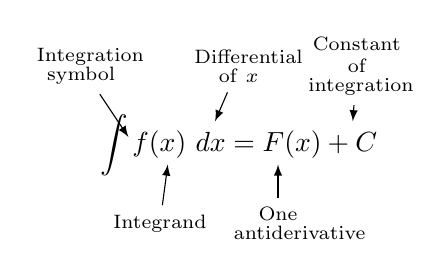
\begin{tikzpicture}[>=latex]
%\draw [thin,step=1cm] (0,0) grid  (3,3);
\draw  (2,2) node {$\displaystyle \int f(x)\ dx=F(x)+C$};

\draw [{\colorone}] (1,1) node [](a) {\scriptsize Integrand};
\draw [{\colorone},->] (a) -- (1.1,1.75);

\draw [{\colorone}] (0,3) node [text width=32pt,align=center] (b) {\scriptsize \centering Integration\\[-5pt] symbol};
\draw [{\colorone},->] (b) -- (.6,2.1);

\draw [{\colorone}] (2,3) node [text width=32pt,align=center] (c) {\scriptsize \centering Differential\\[-5pt] of $x$};
\draw [{\colorone},->] (c) -- (1.7,2.3);

\draw [{\colorone}] (2.5,1) node [text width=32pt,align=center] (c) {\scriptsize \centering One\\[-5pt] antiderivative};
\draw [{\colorone},->] (c) -- (2.5,1.75);

\draw [{\colorone}] (3.5,3) node [text width=35pt,align=center] (c) {\scriptsize \centering Constant of\\[-5pt] integration};
\draw [{\colorone},->] (c) -- (3.45,2.3);



\end{tikzpicture}
